%% Copernicus Publications Manuscript Preparation Template for LaTeX Submissions
%% ---------------------------------
%% This template should be used for copernicus.cls
%% The class file and some style files are bundled in the Copernicus Latex Package, which can be downloaded from the different journal webpages.
%% For further assistance please contact Copernicus Publications at: production@copernicus.org
%% https://publications.copernicus.org/for_authors/manuscript_preparation.html


%% Please use the following documentclass and journal abbreviations for preprints and final revised papers.

%% 2-column papers and preprints
\documentclass[amt]{copernicus}



%% Journal abbreviations (please use the same for preprints and final revised papers)

%% \usepackage commands included in the copernicus.cls:
%\usepackage[german, english]{babel}
%\usepackage{tabularx}
%\usepackage{cancel}
%\usepackage{multirow}
%\usepackage{supertabular}
%\usepackage{algorithmic}
%\usepackage{algorithm}
%\usepackage{amsthm}
%\usepackage{float}
%\usepackage{subfig}
%\usepackage{rotating}

\newcommand{\todo}[1]{{\color{red} #1}}

\begin{document}

\title{Cloud correction and filtering of operational microwave humidity
  radiances with case specific uncertainty estimation}


\Author[1]{Inderpreet}{Kaur}
\Author[1]{Patrick}{Eriksson}
\Author[1]{Simon}{Pfreundschuh}

\affil[1]{Department of Space, Earth and Environment, Chalmers University of
  Technology, Gothenburg, Sweden} 

%% If authors contributed equally, please mark the respective author names with an asterisk, e.g. "\Author[2,*]{Anton}{Aman}" and "\Author[3,*]{Bradley}{Bman}" and add a further affiliation: "\affil[*]{These authors contributed equally to this work.}".


\correspondence{Inderpreet Kaur <kauri@chalmers.se>}

\runningtitle{Cloud correction with case specific uncertainty estimation}

\runningauthor{Kaur et al.}

\firstpage{1}

\maketitle


\begin{abstract}
TEXT
\end{abstract}


\copyrightstatement{TEXT}


\introduction
%
Satellite observations of humidity inside the troposphere are mainly performed
by downward-looking sensors. Among this class of observations, the frequency
range around 183\,GHz has a special position. Water vapour has a noticeable
transition at 22\,GHz, but it is relatively weak and only column values can be
derived \citep[e.g.][]{schluessel1990atmospheric} for the observation geometry
of concern. The first transition in the microwave region that can be used to
derive altitude information, i.e.\ can be used for ``sounding'', is the one at
183.31\,GHz \citep{kakar1983retrieval,wang1983profiling}. On the other hand, at
infrared wavelengths a high number of water vapour transitions are found,
including some of high strength. As a consequence, infrared sounders can
provide humidity profiles with high precision and good vertical resolution, but
with strong limitations imposed by clouds. To be able to also sense humidity
inside and below clouds weather satellites are since some time equipped with
channels around 183\,GHz. Today such channels are part of several sensors, such
as ATMS (Advanced Technology Microwave Sounder, \citet{weng2012introduction}).

Precipitation and most dense clouds, particularly if found at high altitude, can
still affect measured radiances around 183\,GHz
\citep[e.g.][]{bennartz2003sensitivity}. As the impact from the hydrometeors
then is dominated by scattering, the complexity of the analysis of the data
increases dramatically and there exists a need to identify the problematic
cases. This is normally denoted as cloud filtering, to obtain data of ``clear
sky'' character. Such filtering has been applied to derive climate records
\citep{lang2020new} and is essential in studies of the agreement between
observations and simulations \citep{brogniez2016review} as well as 
comparing observations of different instruments to validate their calibration
\citep{john2013assessment,moradi:retri:15,berg2016intercalibration}. A commonly
used cloud filtering methods for these applications is the one of
\citet{buehler:aclou:07}. This method is based on the 183\,GHz data alone,
involving rules on the brightness temperatures differences between channels. An
older version is \citet{burns1997effects}.

The main motivation for introducing 183\,GHz channels in operational sensors is
numerical weather prediction (NWP). Usage of microwave data by ``all-sky''
assimilation is growing \citep{geer2017growing}, but 183\,GHz data are still
mainly used in a clear sky fashion \citep{geer2018all}. The later is
particularly true in NWP of regional scope, all-sky assimilation of 183\,GHz at
many national weather agencies will likely not be reached in many years. The
cloud filtering in NWP differs between centres. One approach is to make use of
a ``scattering index'' \citep{bennartz2002precipitation}, based on the
observations alone. Today, likely more common is to use ``observation minus
background'' (O-B), where the forecast model is used to obtain an estimate of
the expected clear-sky value and the observation is rejected if the deviation
exceeds some threshold (???). In both cases, the filtering typically involves
observations around 89 and/or 150\,GHz.

Despite the broad usage these filtering methods have some drawbacks. For
183\,GHz, the impact of hydrometeors systematically causes a decrease in the
observed radiance (maybe with exceptions at extremely dry conditions), see
e.g.\ \citet{barlakas:three:20} and below. This means that if any cloud
contamination is missed by the filtering this will cause a negative bias in
mean radiance, compared to the true clear-sky mean. This bias will translate to
a bias in humidity after the retrieval or assimilation. The alternative is to
apply a very strict filtering, but this will result in that a high fraction of
actually clear-sky values will be rejected \todo{(Reka or better reference)},
i.e.\ an important loss of useful data.

The filtering is normally done in a ``one for all'' manner, i.e.\ all 183\,GHz
channels are either kept or rejected, while, as the channels differ in their
altitude coverage, there could be cloud impact in some channels and still the
others can be considered as clear-sky. To allow a channel specific filtering,
data likely need to be combined in a more complex manner than simple
differences, but it is unclear what type of regression that would be best. This
points towards applying machine learning, as used by e.g.\
\citet{favrichon2019detecting}.

A maybe less obvious problem is the uncertainty to assign to the filtered
values. To our best knowledge, in best case estimates of mean and worst case
errors are provided. Some cases with relatively high cloud impact will likely be
missed, while most cases are clear sky from start. As the remaining cloudy
cases can cause significant biases, the likely solution is to apply a quite
conservative (high) error estimate. However, this will unnecessary downgrade
the value of the truly clear sky cases and the observations are used in a
non-optimal manner.

We are here approaching cloud filtering task from a new angle. The basic idea
is to derive an estimate of the corresponding noise-free clear-sky (NFCS) value
(i.e.\ the radiance that would have been measured in absence of noise and
hydrometeors). This is done for each channel separately, only using
measurements (no ``background'' data involved). Not only a best estimate is
provided, but also a case specific uncertainty.

This information can be used as a pure filter, by rejecting data where the
correction exceeds some threshold value. This threshold value should be
relatively low, to not introduce a bias in filtered dataset. However, even
better is to replace the original value with the predicted NFSC value when
forming the clear-sky dataset. This approach we denote as cloud correction. It
is shown below that a basically bias free cloud correction can be obtained.
This feature removes the need of threshold value, as long as the retrieval or
assimilation system can incorporate the uncertainty of the corrected value. As
also will be shown, the uncertainty for originally clear sky data is determined
by noise, but the uncertainty increases with magnitude of correction.
Accordingly, the cloud correction approach allows that the full weight of
clear-sky data can be preserved.

The estimation of NFSC values makes use of a special type of machine learning,
denoted as Quantile Regression Neural Network (QRNN,
\citet{pfreundschuh:aneur:18}). Unlike standard usage of machine learning where
only some kind of best estimate is provided, QRNN works in a Bayesian fashion
and instead gives a description of the posterior uncertainty. More precisely,
QRNN outputs an user specified set of percentiles that gives a discrete
description posterior distribution, that can be process to derive e.g.\ the
expectation value.

The approach is demonstrated on a combination of 183\,GHz channels (following
\citet{buehler:aclou:07}), but we mainly explore the cloud correction (of
183\,GHz data) that will be possible when sub-millimetre data will be at hand
in some years. This wavelength region will be introduced by the Ice Cloud
Imager (ICI, \citet{eriksson:towar:20}), but likely also be included in several
smaller missions (such as AWS presented below). The focus on ICI is motivated
by several reasons. The true potentail of the QRNN cloud correction approach is
likely not revealed if tested on existing data and applying ICI data for cloud
filtering has not earlier been discussed. It is also argued that the cloud
correction makes it possible to make good use of ICI data already in clear-sky
assimilation, a fact that should speed up the use of this novel data source.



\newpage

\section*{Outline of sectioning}

2 Data and methods

2.1 Satellite sensors

2.1.1 Ice Cloud Imager (ICI)

2.1.2 Microwave Imager (MWI)

2.1.3 Arctic Weather Satellite (AWS)

2.2 Quantile Regression Neural Network (QRNN)

2.2.1 Theory

2.2.2 Evaluation metrics

2.3 Simulations

2.3.1 Input data

2.3.2 Simulation setup

2.3.3 Produced dataset
(If diifers between ICI, MWI and AWS, clarify this)

\noindent 3 Results

Short recap of aim of correction. We also use the correction as a filter, using
a threshold on the correction. We use 5K (?) threshold as example.

3.1 QRNN network configurations and training

3.2 ICI

3.2.1 Example results

Show a few estimated posterior distributions (one figure) and distribution of
predicted values (Fig 2)

3.2.2 Error of best estimate

3.2.3 Predicted uncertainty

3.3 MWI

3.3.1 MWI alone

Just 183 GHz channels, original noise

3.3.2 MWI and ICI

As in present version

3.4 AWS

\noindent 4 Discussion

\noindent 5 Conclusion


\newpage
\section{Data and methods}



\subsection{Ice Cloud Imager}
%
%t
\begin{table*}[t]	
	\caption{Specifications of ICI and MWI channels. For MWI only 183\,GHz channels are shown.}
	\label{tab:ICI_MWI_channels}
	\begin{tabular}{lrrrr}
		\tophline
		Channel & Frequency 	& Bandwidth  	&NE$\Delta$T	&Polarisation\\
		\middlehline
		I1V&	183.31$\pm$7.00    & 2.0 			& 0.8 		& V\\
		I2V&	183.31$\pm$3.40    & 1.5 			& 0.8 		& V\\
		I3V&	183.31$\pm$2.00    & 1.5 			& 0.8 		& V\\
		I4V&	243.20$\pm$2.50    & 3.0 			& 0.7 		& V\\
		I4H&	243.20$\pm$2.50    & 3.0 			& 0.7 		& H\\
		I5V&	325.15$\pm$9.50    & 3.0 			& 1.2 		& V\\
		I6V&	325.15$\pm$3.50    & 2.4 			& 1.3 		& V\\
		I6V&	325.15$\pm$1.50    & 1.6 			& 1.5 		& V\\
		I8V&	448.00$\pm$7.20    & 3.0 			& 1.4 		& V\\
		I9V&	448.00$\pm$3.00    & 2.0 			& 1.6 		& V\\
		I10V&	448.00$\pm$1.40    & 1.2 			& 2.0 		& V\\
		I11V&	664.00$\pm$4.20    & 5.0 			& 1.6 		& V\\
		I11H&	664.00$\pm$4.20    & 5.0 			& 1.6 		& H\\		
		\bottomhline
	\end{tabular}
	\begin{tabular}{lrrrr}
		\tophline
		Channel & Frequency 	& Bandwidth  	&NE$\Delta$T	&Polarisation\\
		\middlehline
		MWI-14&	183.31$\pm$7.00    & 2.0 			& 1.3 		& V\\
		MWI-15&	183.31$\pm$6.10    & 1.5 			& 1.2 		& V\\
		MWI-16&	183.31$\pm$4.90    & 1.5 			& 1.2 		& V\\
		MWI-16&	183.31$\pm$3.40    & 1.5 			& 1.2 		& V\\
		MWI-16&	183.31$\pm$2.00    & 1.5 			& 1.3 		& V\\	
		\bottomhline
	\end{tabular}
	\belowtable{} % Table Footnotes
\end{table*}
Ice Cloud Imager (ICI) is a new EPS-SG (EUMETSAT Polar System - Second Generation) sensor that will observe  Earth using submillimeter-wave (sub-mm) frequency range. The main objective of ICI is measure ice cloud properties and improve the representation of clouds in regional and global models. ICI is a conically scanning millimetre/sub-millimetre radiometer which will measure 13 frequencies from 183 GHz up to 664 GHz. Channels with centre frequencies 183.31, 325.15 and 448.0\,GHz are centered on water vapor absorption lines, and measure vertical polarization. While other channels around 243.0 and 664.0\,GHz are ``window channels'' and receive both vertical and horizontal polarization. 
In addition to ICI, the EPS-SG satellite will also have Microwave Imager (MWI) onboard. MWI will measure frequencies from 18.7 GHz up to 183\,GHz and provide data continuity to the existing microwave imager measurements. The common 183\,GHz channels among the two instruments shall allow cross-calibration between the two instruments. The channel configurations for ICI and MWI (only 183\,GHz) are provided in Table~\ref{tab:ICI_MWI_channels}.

\subsection{ICI simulations}
\label{sec:arts_simulations}
%

**** Some parts copied directly from AWS report *****

The satellite observations for all ICI channels are simulated with the Atmospheric Radiative Transfer Simulator (ARTS, (ARTS, \citet{eriksson:arts2:11,buehler:artst:18})version. The simulations include TB from five ICI channels around 183\,GHz, 243\,GHz, 325\,GHz, 448\,GHz and 664\,GHz. 

The absorption model takes into account the effect from nitrogen
\citep{pwr:93}, oxygen \citep{pwr:93} and water vapour
\citep{ellison2007permittivity}. LWC is taken from ERA-Interim and is assumed
to be totally absorbing. In the mapping of CloudSat reflectivities to RWC and
IWC a total separation between liquid and ice phase is assumed. All scattering
hydrometeors at temperatures above 0$^\circ$C are assumed to be rain, and all
below 0$^\circ$C are assumed to be ice hydrometeors. For RWC the particle size
distribution of \citet{abel2012improved} is applied. The PSD of IWC follows the
basic formulation applied in DARDAR (\verb
 http://www.icare.univ-lille1.fr/projects/dardar), using latest parameter
 values (i.e.\ $\alpha$ and $\beta$) as given by \citet{cazenave2019evolution}.
 This PSD can be considered as a ``two moment'' scheme, but is here applied in
 a one moment manner by setting $N_0^*$ (as a function of temperature)
 following Table~5 of \citet{delanoe2014normalized}, and letting the radar
 reflectivity set the remaining moment. Single scattering data are taken from
 \citet{eriksson:agene:18}. For ice hydrometeors, three habits are applied:
 Perpendicular 3-bullet rosette, Large plate aggregate and Large column
 aggregate. In the last two cases, the aggregates are complemented with single
 crystal data to also cover smaller sizes. These data describe particles
 assumed to have a totally random orientation. To apply oriented particles is
 much more computationally costly and could not be accommodated inside the
 study. The land emissivity was taken from TELSEM \citep{aires2011tool} and the
 Ocean/water from TESSEM \citep{prigent2017sea}. For each atmopsheric case,
 both ''clear-sky'' and ``all-sky'' calculations were performed. In the former,
 all impact of all hydrometeors were set to zero, while in the latter, IWC and
 RWC derived from CloudSat reflectivities and LWC from ERA-Interim were taken
 into account. Both sets of calculations were made by ARTS's interface to the
 RT4 solver \citep{evans1995microwavec}. To avoid a possible bias between
 clear-sky and all-sky for insignificant hydrometeor contents, the same
 ``scattering solver'' was used for both calculations. The first two elements
 of the Stokes vector were calculated.

\subsection{Simulation dataset}
%
Using the simulation setup described in previous section, Cloudsat profiles during August 2015 were randomly selected to generate 200\,000 cases for each ICI frequency. The input data were restricted between $60^{\degree}$S to $60^{\degree}$N, and surface is below 500\,m. Both clear-sky and all-sky scenarios were simulated, and no differentiation was made between the observations over ocean/sea and land. It is also assumed that all simulations are remapped to a common foorprint. 

**** show any comparsion to ATMS? or AWS channels ? ****

\subsection{QRNN}
%
The neural network training is a process of learning to predict the outputs {$y_i$} from inputs {$x_i$} through a series of learnable transformations. While training, neural networks seek to minimise the model error through a loss function. The choice of the loss function depends on the predictive problem. When a neural network is trained to minimise the mean of the quantile loss function to predict the quantiles of the distribution, it is called a Quantile Regression Neural Network (QRNN). 

 
\subsubsection{Model selection}
%
\label{model_selection}
A high performing QRNN model requires tuning of multiple hyper-parameters. These parameters determine the structure and the training set-up of the neural network. Several of these hyper-parameters are non-learnable, and must be defined before beginning of every training. Grid search is one of the most often employed techniques for hyper-paramter tuning. In grid search, different combinations of hyperparamters are selected and for each, the model performance is evaluated. The model architecture with the best performance is selected. The model evaluation metrics employed in this article are described in the next section. 

For the structural parameters, the grid search is performed to determine the number of neurons (width) and hidden layers (depth). The model is trained for multiple values of layer widths and hidden layers, and the best configuration is selected by evaluating the predictions over the validation set. Similarly, the training process is optimized by performing a grid search different training parameters such as : batch size, learning rate, number of epochs, decay. The best performing hyperparameter configurations for a particular training set need not be same for other datasets. Therefore for each QRNN model used in this article, the hyperparameters were tuned distinctly. 

\subsubsection{Evaluation metrics}

Quantile loss function

CRPS


\section{Cloud correction in  183 GHz channels}
%
\subsection{Training data}
%
Out of the 200\,000 ICI and MWI channel simulations, 150\,000 cases are randomly picked to form the training set. The rest are used for testing. In the training set, 90\% of the data is randomly selected to form the training set, while the other 10\% form the \textit{testing-during-training} database. ARTS simulations are noise free, so to incorporate the satellite measurement uncertainties, gaussian noise is added to the input training data according to the channel NE$\Delta$T. The target training data is kept noise free. In order to build a robust learning network, random noise is added to the inputs at each training iteration. This exposes the model to a different datasets during the entire training process and avoids the memorisation of training samples. The input data is also normalized with mean and standard deviation.
It is assumed for the simulations that the ICI and MWI channels are mapped to a common footprint and resolution. In such case, remapping reduces the noise in MWI channels from 1.2\,K at 10\,Km resolution to 0.8\,K at 15\,Km resolution.
\subsection{Training}
\label{sec:ici_trainin}
%t
\begin{table}[t]
\caption{Summary of the different QRNN models used in the study.}
\label{tab:QRNN_models}
\begin{tabular}{lll}
\tophline
QRNN model & Training inputs & Target \\
\middlehline
QRNN-simple & I1V, I5V, I6V, I7V, I8V, I9V, I10V, I11V 			 & I1V\\
			& I2V, I5V, I6V, I7V, I8V, I9V, I10V, I11V 			 & I2V\\
			& I3V, I5V, I6V, I7V, I8V, I9V, I10V, I11V 			 & I3V\\
			& MWI-15, I5V, I6V, I7V, I8V, I9V, I10V, I11V 		 & MWI-15\\	
			& MWI-16, I5V, I6V, I7V, I8V, I9V, I10V, I11V 		 & MWI-16\\
QRNN-all    & I1V, I2V, I3V, I5V, I6V, I7V, I8V, I9V, I10V, I11V & I1V\\	
			& I1V, I2V, I3V, I5V, I6V, I7V, I8V, I9V, I10V, I11V & I2V\\	
			& I1V, I2V, I3V, I5V, I6V, I7V, I8V, I9V, I10V, I11V & I3V\\
			
\bottomhline
\end{tabular}
\belowtable{} % Table Footnotes
\end{table}
To investigate the performance of training inputs, two QRNN models with different set of training inputs are analysed. In both models, the training set combines data from 183\,GHz, 325 GHz, 448\,GHz and 664\,GHz to predict cloud corrected observations for the target 183\,GHz channel.

In the first model, the training set includes the target 183\,GHz channel and the sub-mm channels. For example, to train for channel I1V, the input channels are I1V, I5V , I6V, I7V, I8V, I9V, I10V, I11V. A separate QRNN model is trained for each of the 183\,GHz channels. We shall refer this QRNN model as ``QRNN-simple''. In the second QRNN model, we suggest to use all three 183\,GHz channels (from ICI) concurrently, along with sub-mm channels. In this case, although the input training parameters are identical for all channels, the target channel is different and QRNN has to be trained separately for each. Further in text, we refer this model as ``QRNN-all''. Table~\ref{tab:QRNN_models} summarises the two QRNN models. 
   
Apart from these two models, we also extend QRNN-simple to predict the clear-sky values for MWI channels. In this case, we combine the measurements from MWI-15(MWI-16) and the sub-mm channels to predict MWI-15(MWI-16). Since we assume that all channels are remapped to a common footprint, channels MWI-14, MWI-17 and MWI-18 are virtually identical to I1V, I2V and I3V, and thus results for them are not shown separately. 

As described in section \ref{model_selection}, a grid search was implemented to select the best performing hyperparamters. The mean quantile loss and CRPS for different layer width and hidden layer configurations are shown in Fig\ref{fig:model_selection}. The results are for QRNN-simple with I3V as target channel. Increasing the complexity of the network by increasing the layer-width and depth has a positive impact on performance. However for four hidden layers, increasing the number of neurons beyond 128 has no significant impact on the performance. On basis of these results, a neural network with four hidden layers and 128 neurons in each layer was selected for QRNN-simple. For the optimising the training paramters, a customised  learning rate scheduler was implemented. The initial learning rate was reset after a certain number of epochs.  We started the training process with a initial learning rate of 0.1, and decreased it by a factor of 10 after 100 epochs. The best neural network performance was obtained when the network was trained three times with a new initial learning rate. For each training  if the validation loss remained unchanged till 6 training epochs, the learning rate was reduced by a factor of 2. We did not optimise the type of activation function and batch size. Rectified Linear Unit (ReLU) was used as the activation function  and the batch size was set to 128 samples for all QRNN models. 

For QRNN-all a grid search (results not shown) over width and depth and learning rates resulted in similar performance, and an identical neural network was selected.

\begin{figure}[t]
	\centering
	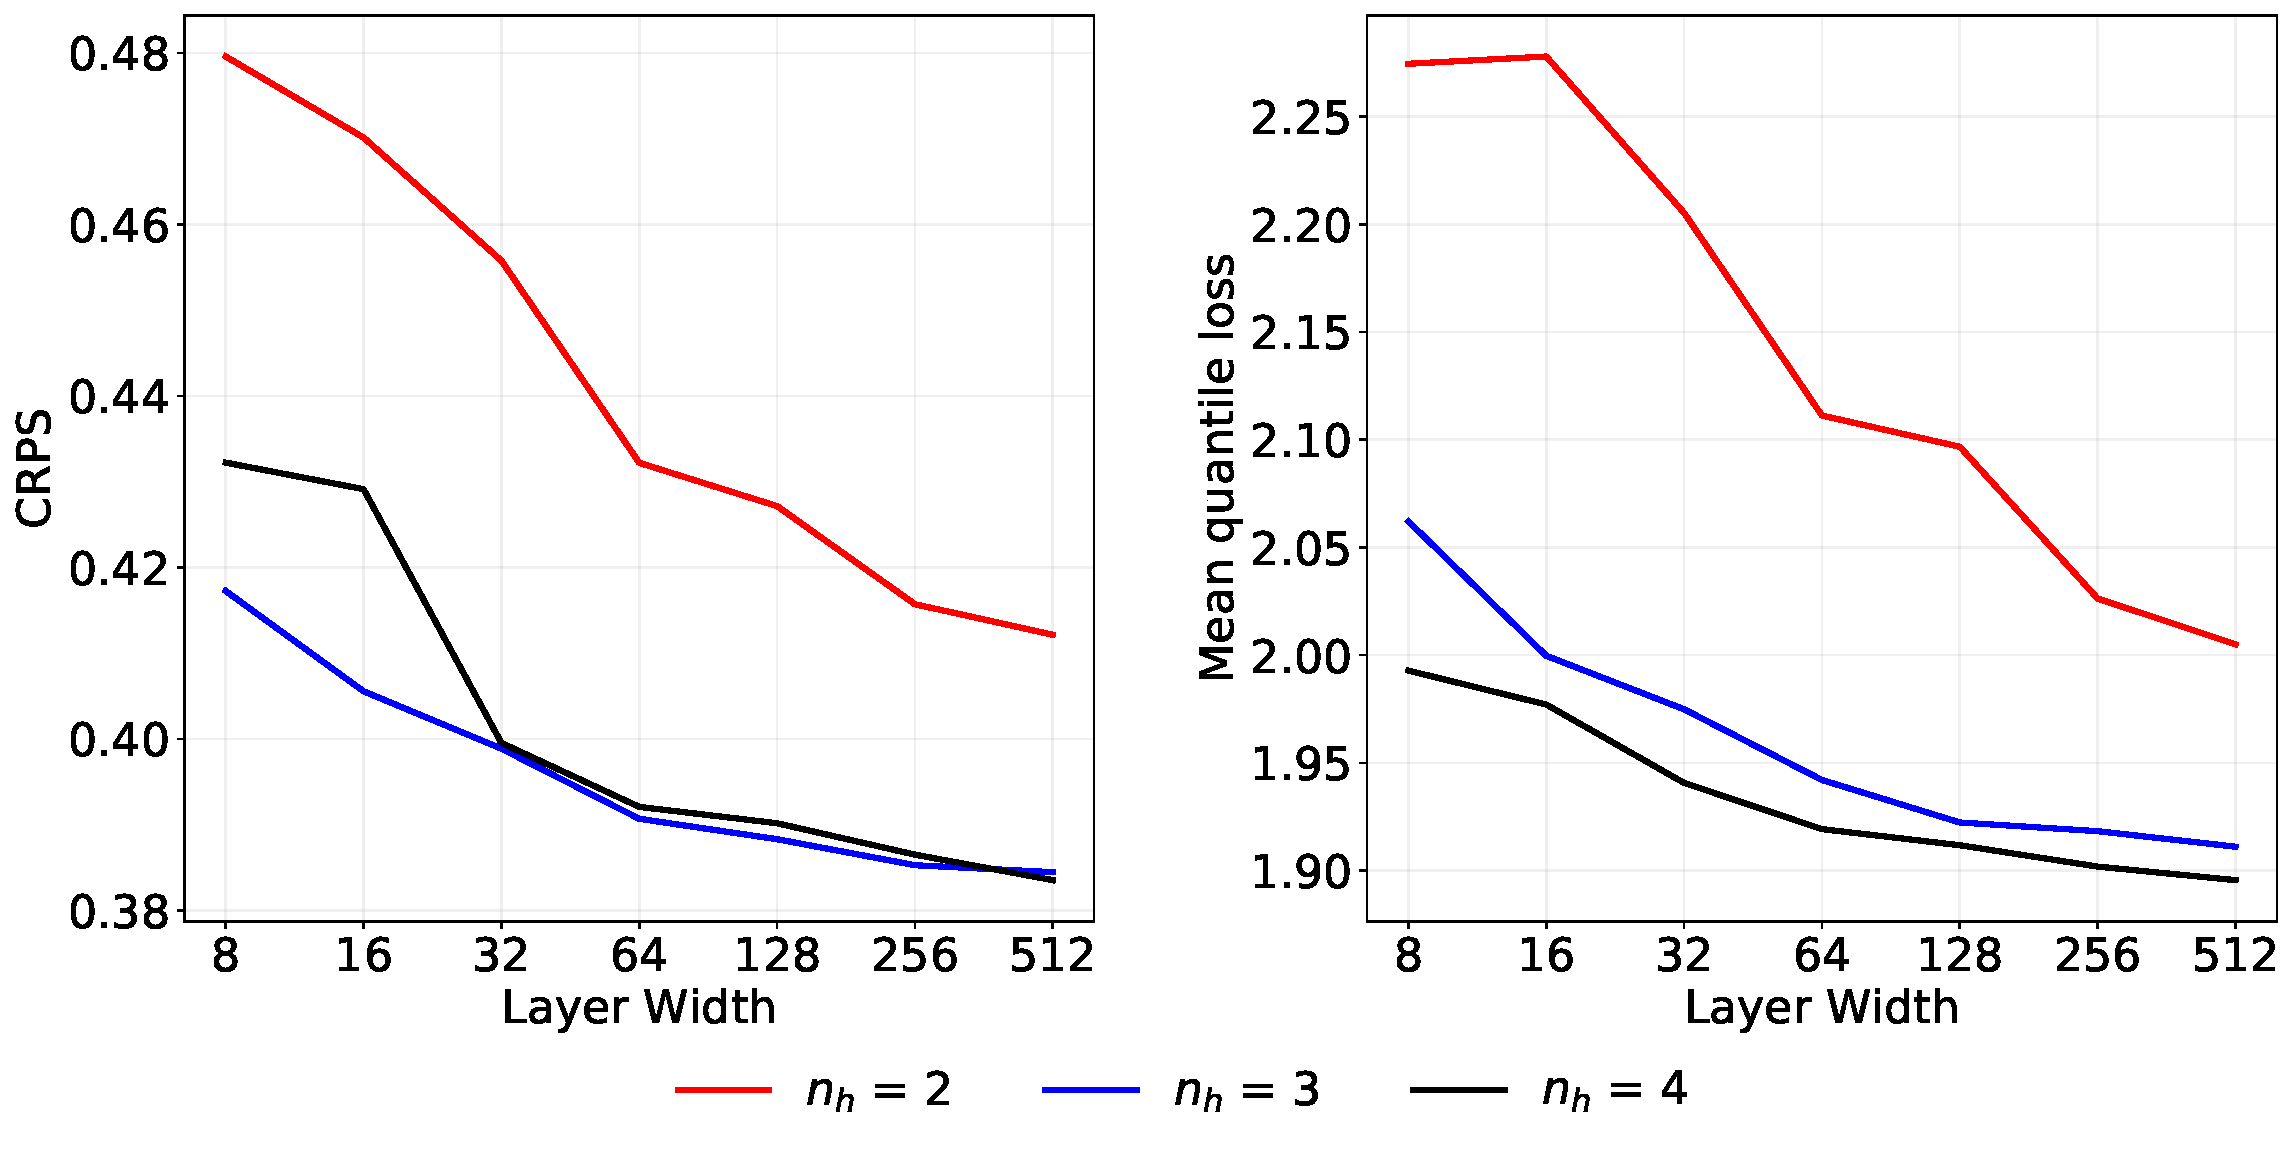
\includegraphics[height=60mm]{Figures/CRPS.pdf} 
	\caption{CRPS(left) and mean quantile loss(right) for different combinations of layer width and hidden layers ($n_h$). The results are from QRNN-simple for channel I2V.}
	\label{fig:}	
\end{figure}

\subsection{Results}
%
%f 
\begin{figure}[t]
	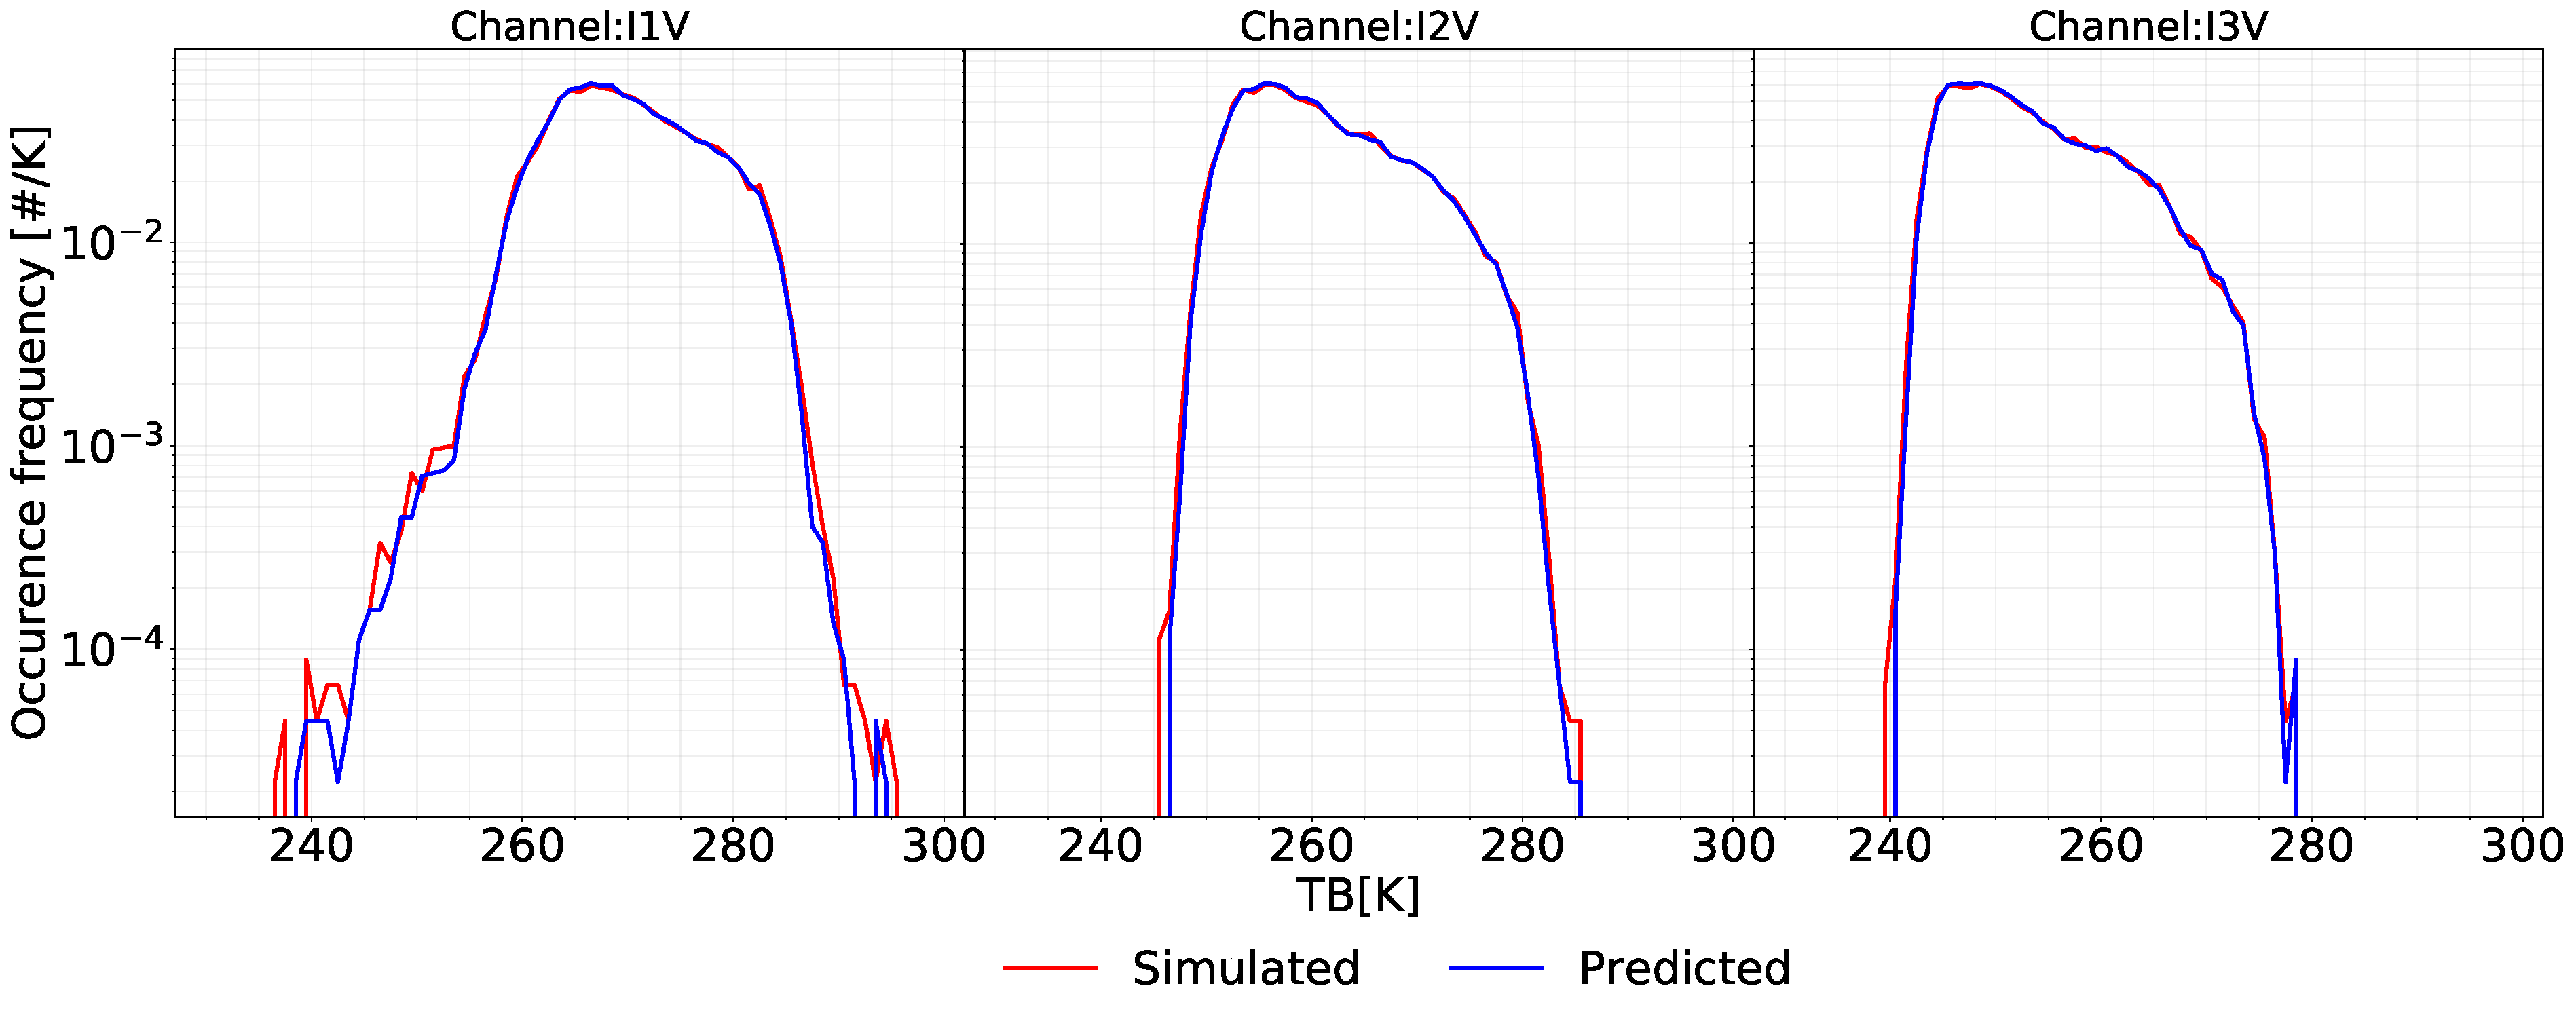
\includegraphics[width=\textwidth]{Figures/PDF_predictions_ICI.pdf} 
	\caption{Distributions of predicted clear-sky values from QRNN-simple for channels I1V, I2V and I3V. }
	\label{fig:PDF_predictions}	
\end{figure}
%f 
\begin{figure}[t ]
	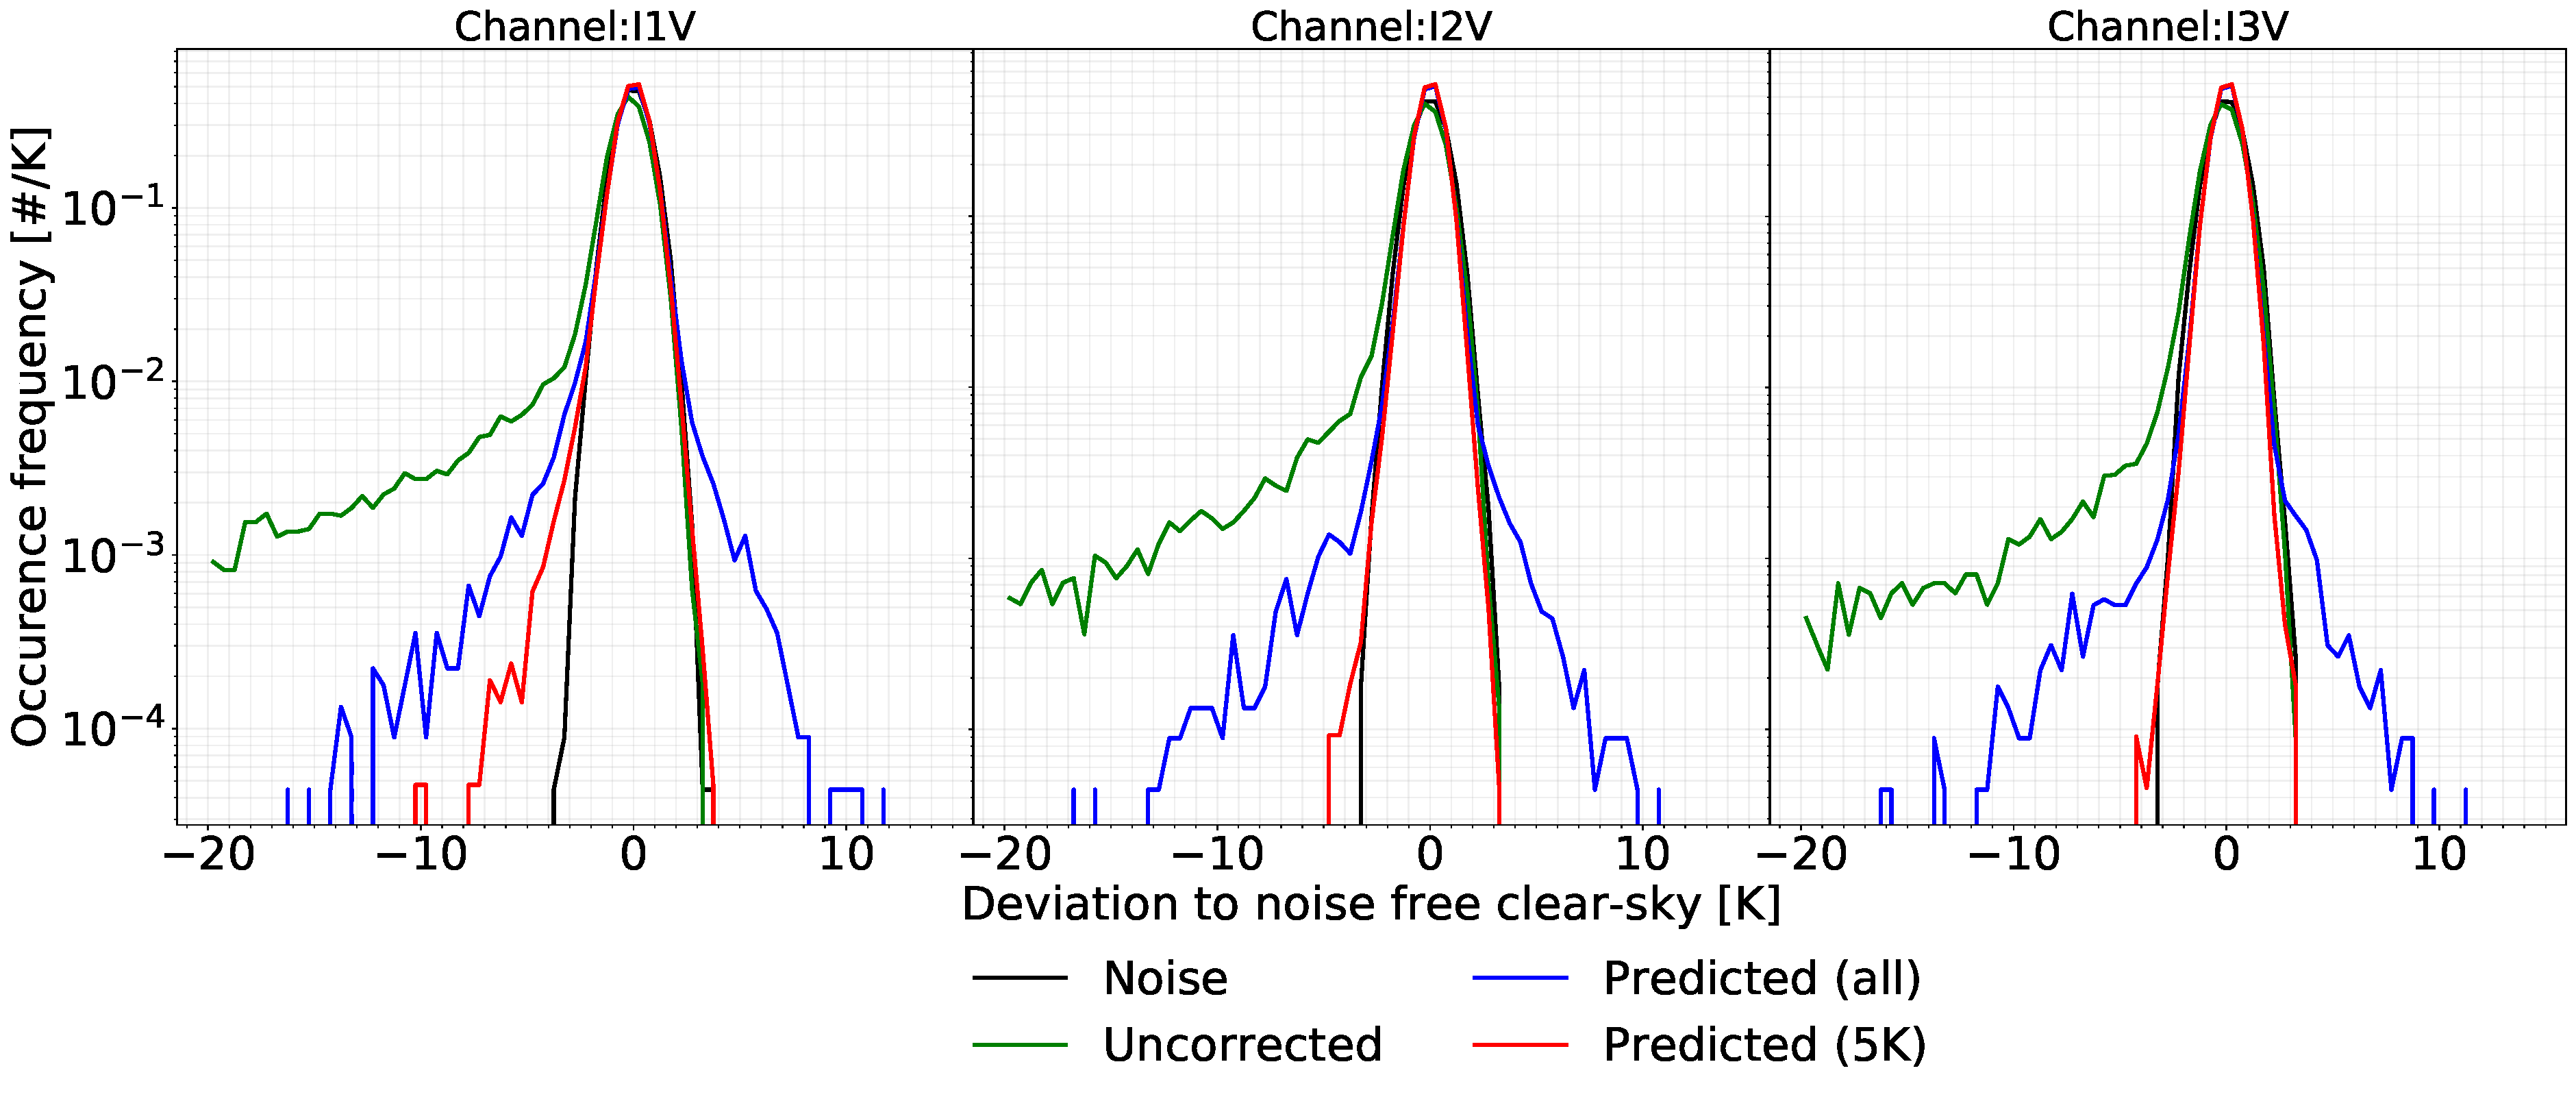
\includegraphics[width=\textwidth]{Figures/error_distribution_QRNN-single.pdf} 
	\caption{Error distributions for deviations of QRNN-simple predictions to clear-sky simulations for channels I1V, I2V and I3V. Label ``uncorrected'' represents the measurements, ``predicted'' denotes the entire dataset, while ``predicted(5\,K)'' refers to the dataset where cases with cloud correction greater than 5\,K are excluded.}
	\label{fig:error_distributions}	
\end{figure}

%t
\begin{table}[t]
	\caption{Bias, mean absolute error(MAE), standard deviation(STD), and measure of skewness(Skewness) for error distributions of predictions of I1V, I2V and I3V. Results from both QRNN-simple and QRNN-all are shown. The label ``All'' refers to the complete dataset, while in ``Filtered'', cases with cases with cloud correction greater than 5\,K(15\,K) are excluded from statistics. The fraction of cases removed by this filter are given in parentheses.}
	\label{tab:error_statistics_ici}
%	\tabcolsep=0.11cm
	\begin{tabular}{llrr|rrr|rrr}
		\tophline
		&&\multicolumn{2}{c|}{Simulations}& \multicolumn{3}{c|}{QRNN-simple} & \multicolumn{3}{c}{QRNN-all}\\
		\cline{3-10}
%		\hline
		&&   Clear-sky &   All-sky &   All &   Filtered(5K) & Filtered(15K) & All &   Filtered(5K) & Filtered(15K) \\
		\middlehline
%		\multicolumn{7}{c}{Channel - I1V}\\

Channel I1V &Bias     &   -0.00 &   -1.90&    -0.03 &      0.00(6.40\%) & 0.01(3.09\%)&-0.01 &0.01 (6.42\%)& 0.02(3.09\%) \\
			&MAE      &    0.64 &    2.35&     0.69 &      0.60 & 0.63  &  0.65 & 0.62& 0.60\\
			&STD      &    0.80 &    8.92&     1.05 &      0.78 &  0.84 &  0.97 & 0.84& 0.80\\
			&Skewness &   -0.01 &   -7.99&    -1.24 &     -0.44 & -0.48 & -0.36 &-0.51&-0.34\\
\middlehline
Channel I2V	&Bias     &   -0.00 &         -1.05 &    0.02 &      0.03(3.70\%)&0.02(1.60\%) &  0.02&   0.03(3.67\%)& 0.02(1.60\%)\\
			&MAE      &    0.64 &          1.54 &    0.56 &      0.50&  	  0.52 &  0.46&   0.42 &  0.52\\
			&STD      &    0.80 &          5.98 &    0.86 &      0.64&  	  0.69 &  0.70&   0.53 &  0.69\\
			&Skewness &    0.02 &        -10.64 &   -2.25 &     -0.22& 		 -0.58 & -1.69& -0.25 &-0.56\\
\middlehline	
Channel I3V &Bias     &   0.00  &         -0.63 &    0.02 &      0.02(2.18\%)&0.03(0.92\%)&	 0.04 &  0.04(2.18\%) & 0.04(0.92\%) \\
			&MAE      &   0.64  &          1.14 &    0.54 &      0.50		& 0.52&0.48 &    0.44 & 0.46\\
			&STD      &   0.80  &          4.26 &    0.80 &      0.64		& 0.68&0.71 &     0.56 & 0.60\\
			&Skewness &   0.00  &        -13.26 &   -1.40 &     -0.16		&-0.61&-1.41&   -0.11 & -0.77\\	
		\bottomhline
	\end{tabular}
	\belowtable{} % Table Footnotes
\end{table}



%t
\begin{table}[t]
	\caption{Same as Table~\ref{tab:error_statistics_ici}, but for channels MWI-15 and MWI-16. Results are from QRNN-simple.}
	\label{tab:statistics_mwi}
	\begin{tabular}{llrr|rrr}
		\tophline
		&&\multicolumn{2}{c|}{Simulations}& \multicolumn{3}{c}{QRNN-simple} \\
		\cline{3-7}
		%		\hline
		&&   Clear-sky &   All-sky &   		 All &   Filtered(5\,K) & Filtered(15\,K) \\
		\middlehline
 MWI-15 		&Bias     &    0.00 &         -1.19 &           -0.02 &                -0.01(4.41\%) & -0.02(1.87\%)\\
				&MAE      &    0.64 &          1.66 &            0.56 &                 0.49 		 &  0.52\\
				&STD      &    0.80 &          6.21 &            0.84 &                 0.64 		 &  0.69\\
				&Skewness &   -0.02 &         -9.87 &           -1.67 &                -0.29 		 & -0.47\\
		\middlehline
 MWI-16 		& Bias 	   &    0.00 &         -0.80 &           -0.04 &   -0.03(2.85\%) & -0.04(1.15\%)\\
				& MAE      &    0.64 &          1.31 &            0.54 &     0.49		 & 0.51\\
				& STD      &    0.80 &          5.01 &            0.82 &     0.63		 & 0.67\\
				& Skewness &    0.01 &        -12.04 &           -1.94 &    -0.23		 &-0.81\\
		\bottomhline			
	\end{tabular}
	\belowtable{} % Table Footnotes
\end{table}
QRNN predictions are estimates of the posterior distribution over different quantiles: $x_{\tau}$, for median, $\pm 1\sigma$, $\pm 2 \sigma$ and  $\pm 3 \sigma$ ($\tau$ = 0.002, 0.03, 0.16, 0.5, 0.84, 0.97, 0.998). To assess the accuracy of the predictions, the median of the posterior distribution is assumed to be the best estimate for the predicted clear-sky value. The prediction errors are calculated as the deviation of the predictions to their corresponding noise-free clear-sky values. We calculate the mean bias, mean absolute error and standard deviation of the errors. The asymmetry of error distributions around their mean is also calculated through the measure of skewness. In the next sections, we describe the performance of the two QRNN models for ICI and MWI channels.

\subsection{Prediction accuracy}
%
The distributions of median value of clear-sky predictions from QRNN-single are shown in Fig~\ref{fig:PDF_predictions}. The distributions of corresponding clear-sky simulations are also plotted as reference. The three figures correspond to channels: I1V, I2V and I3V. These results show that the clear-sky values predicted by QRNN-single have a very good match for the peak of the distributions, but a slight mismatch is evident towards the tails, where QRNN seems to predict slightly colder/warmer TBs. 

For a quantitative evaluation of how accurate the predictions are, the  deviations of the median values to the clear-sky simulations are computed. Fig~\ref{fig:error_distributions} shows the error distributions of predictions for all three channels. The distribution of noise is also plotted for reference. The error metrics corresponding to these results are provided in Table~\ref{tab:error_statistics_ici}. Without any cloud impact, the error distributions should follow a Gaussian distribution, however the presence of clouds leads to a TB reduction, and introduces a high negative bias among the deviations. Among the three channels, the highest cloud impact is seen in channel I1V. The average bias in channel I1V measurements is -1.89\,K, however the QRNN-single predictions successfully reduces the average deviation to -0.03\,K. The predictions and the observations have a good agreement for the main peak of the distribution, albeit the prediction errors have a sharper peak and a larger spread.  The large spread is representative of the few cases which are either under/over predicted. If all the cases with correction greater than 5\,K are excluded, only a fraction of the total cases (6.42\%) are removed but the variability in predictions errors reduces significantly. This indicates that few cases with high cloud impact could be difficult to train and predict.    

The performance of QRNN-single for I2V and I3V is analogous to I1V, though the accuracy seems to be higher for former. When all predictions are included, the average deviation for both I2V and I3V is -0.02\,K, but few cases with large errors increases the spread of the distributions. As observed for I1V, excluding cases with cloud correction greater than 5\,K removes the cases associated with low accuracy. Interestingly, the resulting spread of errors is also narrower than noise. After filtering, the error standard deviation for both I2V and I3V is 0.64\,K compared to 0.80\,K originating from measurement noise.

The results QRNN-all are also shown in Table~\ref{tab:error_statistics_ici}. Using additional information from other 183\,GHz channels has a definite positive impact on the QRNN training. A marked impact is seen for channel I1V, where the low measure of skewness over the entire test set indicates that the resulting distributions are more symmetric than QRNN-simple. When cases with correction greater than 5\,K are excluded, the variability of errors is smaller than noise. A similar trend is observed for channels I2V and I3V.  

Table~\ref{tab:statistics_mwi} shows the metrics from error distributions for MWI-15 and MWI-16 predictions. Results from only QRNN-simple are shown. As shown above for ICI channels, the performance of QRNN-simple for the two MWI channels is consistent. 
 
\subsection{Uncertainty quantification}
%
%f 
\begin{figure}[t]
	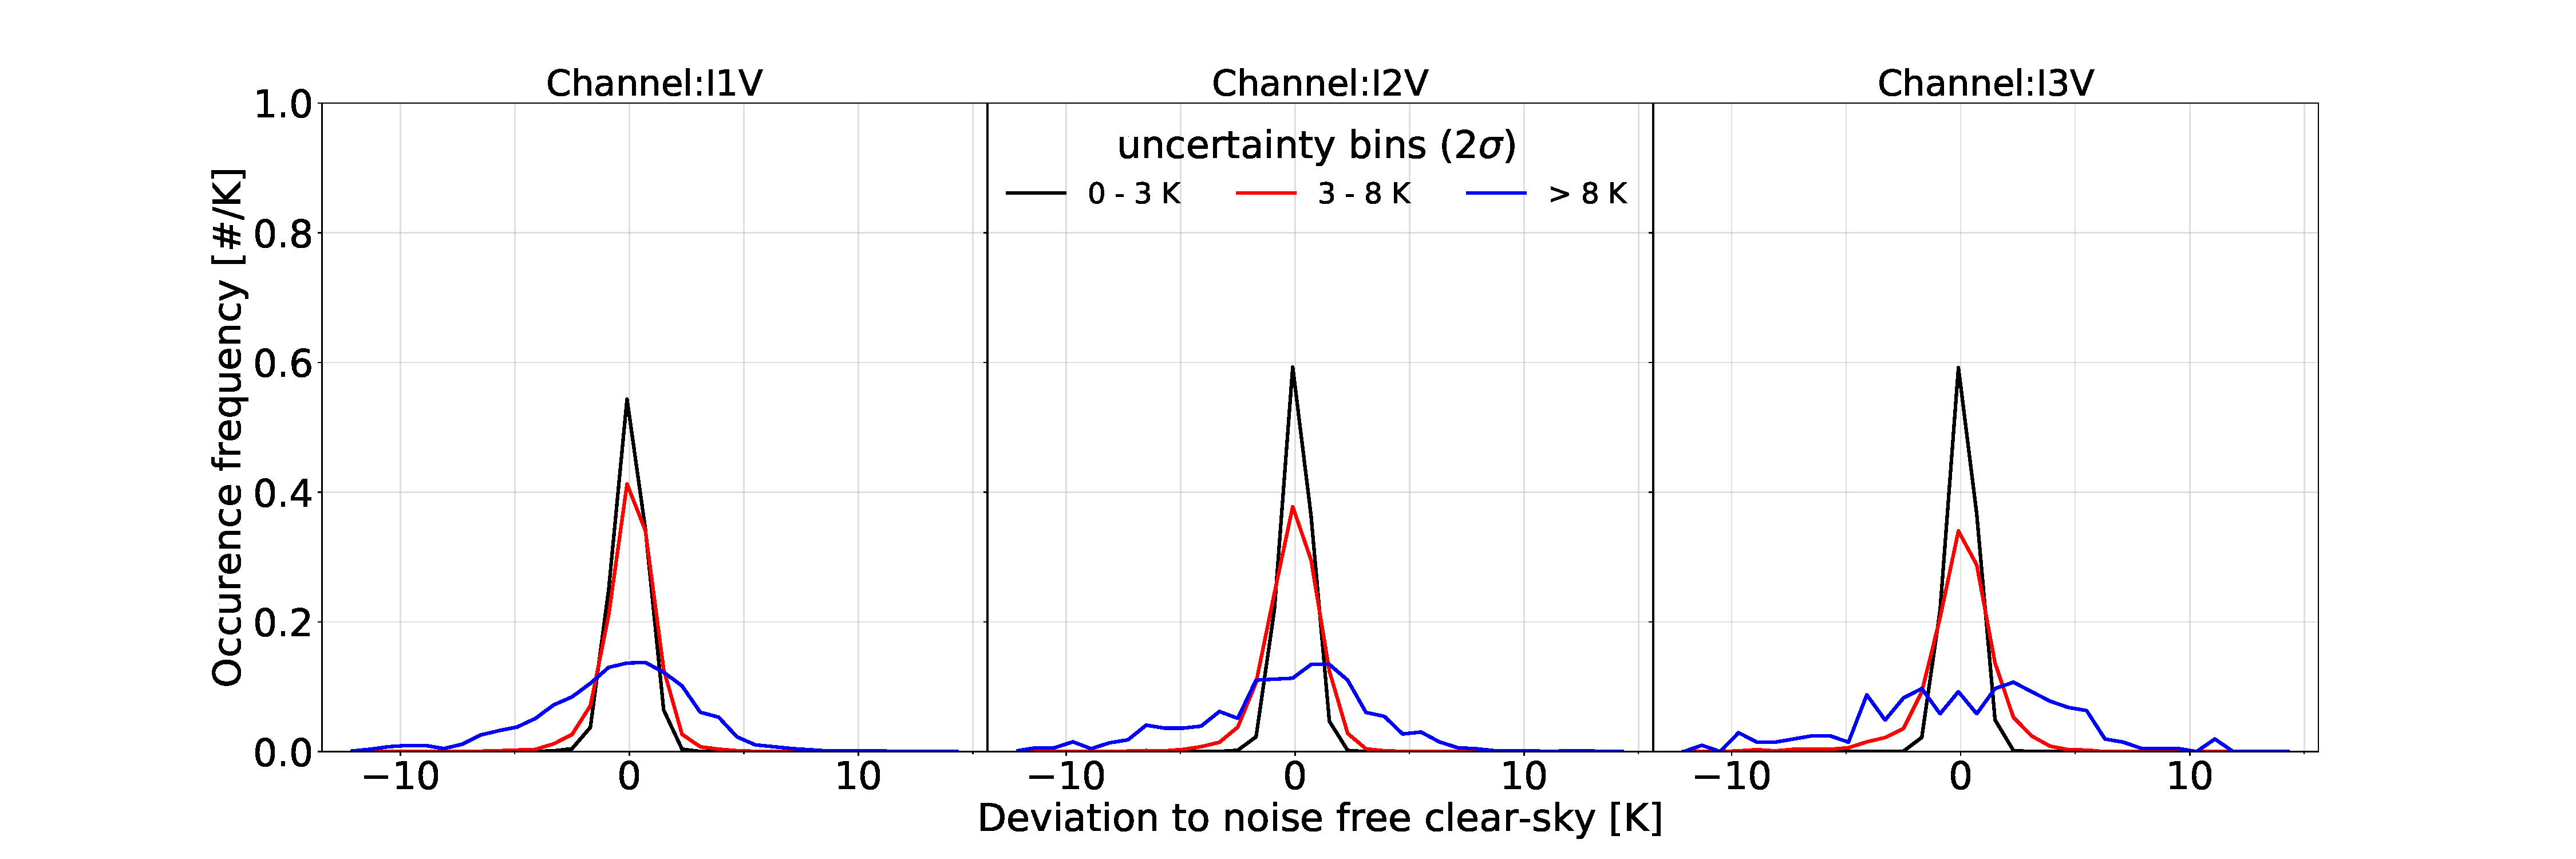
\includegraphics[width=\textwidth]{Figures/PDF_uncertainty_bins_QRNN-single.pdf}	
	\caption{Distribution of errors binned according to their uncertainty. Results are from QRNN-simple for channels I1V, I2V and I3V.}
	\label{fig:error_distribution_uncertainty_bins_I1V}	
\end{figure}
\begin{figure}[t]
	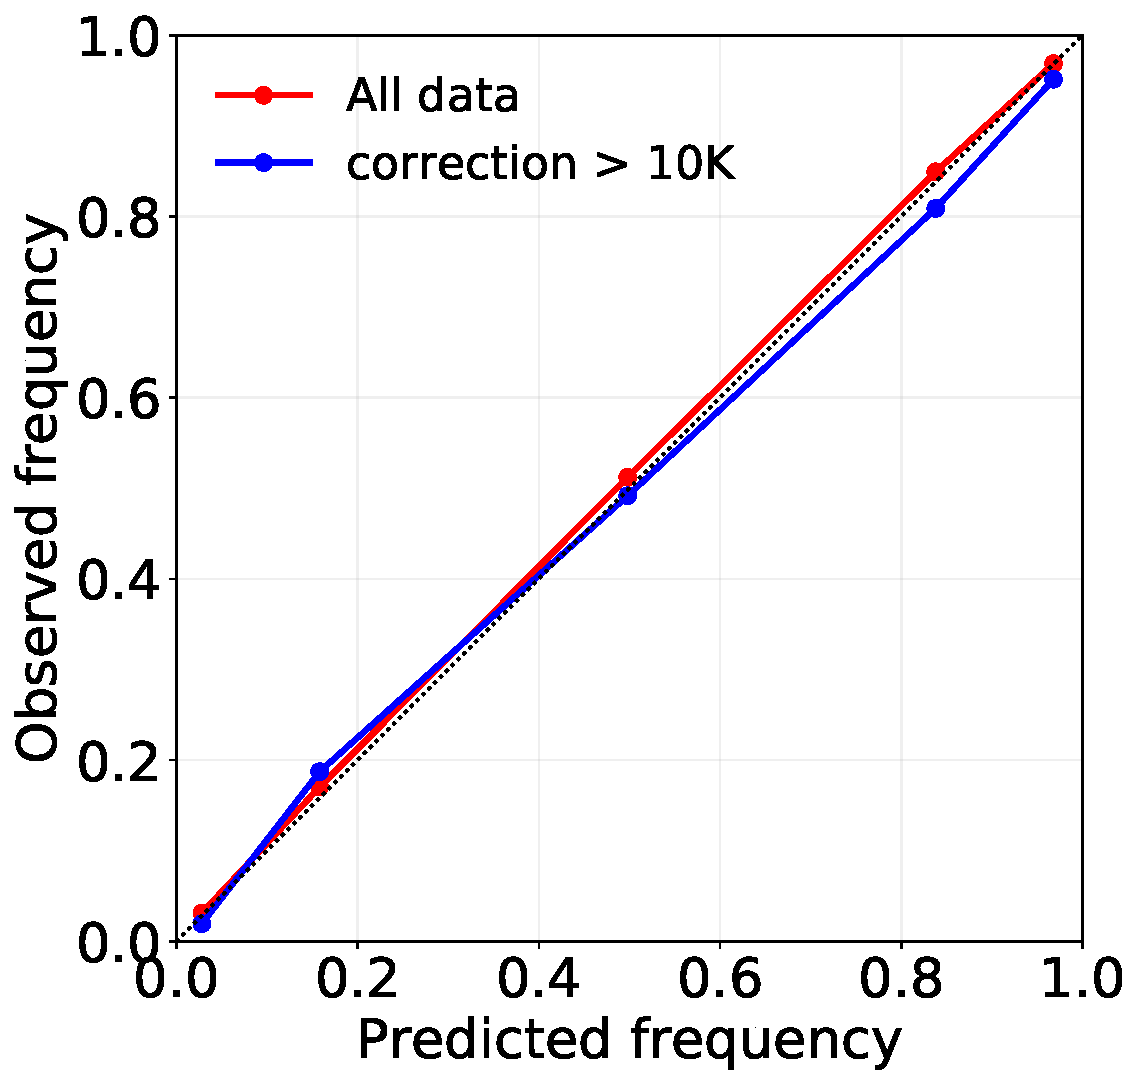
\includegraphics[height = 70mm]{Figures/calibration_QRNN_I2V.pdf}	
	\caption{Calibration of the prediction intervals obtained from QRNN-simple and QRNN-all for channel I2V. }
	\label{fig:calibration_I2V}	
\end{figure}
The biggest advantage of using QRNN is estimation of case-specific uncertainties. The quantiles can be used to construct a probability distribution of the predictions in contrast to other correction approaches which give out only point estimates. The predictions for each quantile can be used to construct the confidence intervals. The confidence interval for each point estimate quantifies it's uncertainty. For example, if $\tau_1$ and $\tau_2$ are two quantiles then there is $\tau_2-\tau_1$ probability that the true value will lie in between the range.

To test if the uncertainty estimates given by QRNN are representative of prediction errors, we divided the $\pm2\sigma$ confidence interval into three bins and estimated the prediction error distribution for each. Fig.~\ref{fig:error_distribution_uncertainty_bins_I1V} shows the prediction error distributions binned according to $2\sigma$ confidence interval for I1V, I2V and I3V. These results are from QRNN-simple. Similar results were also obtained for QRNN-all (figure not shown). Among the three channels the uncertainty in predictions for I1V and I2V are higher than I3V and an increase in the spread of errors with increasing uncertainty is evident in all three. As the errors increase, the spread is mostly symmetric around x-axis but among predictions associated with large uncertainties, high errors occur frequently. In other words, too-low/too-high QRNN predictions tend to be associated with high uncertainty. 

Fig.~\ref{fig:calibration_I2V} shows the calibration of prediction intervals on the test dataset for channel I2V. Results from both QRNN-simple and QRNN-all are shown. The calibration of predictions with correction greater than 5\,K is also shown. For the entire test dataset, the calibration curves for QRNN-simple and QRNN-all are quite identical. If cases with cloud correction greater than 5\,K are considered, the calibration curve for QRNN-simple lies  below y=x line, implying that the prediction intervals are overly narrow. A similar behaviour is observed for channel I3V (figure not shown). However, for channel I1V, both QRNN-all and QRNN-simple fail to provide well calibrated predictions for cases associated with high cloud impact. 

These results show that both QRNN-simple and QRNN-all are successful in providing well calibrated probabilistic predictions of the posterior distributions except for few cases associated with high cloud impact. This is not unexpected, as such cases form a small subset of the training set and their
priori distribution could be different from the the entire dataset. Since such cases form only a fraction of the training dataset, it can be hard to train the model to predict them accurately. A larger training dataset would be required to increase the representation of such cases in QRNN.


\section{Special case of using only 325\,GHz for cloud correction}
In this section, we investigate the possibility of using only channels around
325\,GHz for cloud correction at 183\,GHz. This special case of utilising only
325\,GHz channel can be relevant for smaller satellite missions like Artic
Weather Satellite (AWS) where higher sub-mm channels are not available.

\subsection{Data}
\subsubsection{Artic Weather Satellite}
%t
\begin{table}[t]
	\caption{Specifications of AWS channels around 183\,GHz and 325\,GHz.}
	\label{tab:specifications_AWS}	
	\begin{tabular}{lrr}
		\tophline
		Channel & Frequency 	& Bandwidth  \\
		& [GHz]			& [MHz]		\\
		\middlehline
		AWS-32	&	176.311    & 2000 		\\
		AWS-33	&	178.811    & 2000 		\\
		AWS-34	&	180.311    & 1000 		\\
		AWS-35	&	181.511    & 1000 		 \\
		AWS-36	&	182.311    & \phantom{0}500 	 \\
		AWS-41    & 325.15$\pm$6.60    & 2800 \\
		AWS-42    & 325.15$\pm$4.10    & 1800  \\
		AWS-43    & 325.15$\pm$2.40    & 1200 \\
		AWS-44    & 325.15$\pm$1.20    & \phantom{0}800  \\
		\bottomhline
	\end{tabular}
	\belowtable{} % Table Footnotes
\end{table}

The Arctic Weather Satellite (AWS) is a small satellite mission approved as ESA
Earth Watch Programme Element. It is a small platform carrying a single
across-track scanning microwave radiometer. The main objective of AWS will be
to improve representation of Artic and sub-Arctic weather in NWP models and
improve the global weather forecasts. AWS will will have channels receiving
frequencies around 89\,GHz, 165.5\,GHz, 183\,GHz, 229\,GHz and 325\,GHz. For a
detailed description of the AWS channels see \citet{eriksson2020study}, while a
brief summary of AWS channels relevant to this study are provided in
Table~\ref{tab:specifications_AWS}.

% Let's try avoid citing the AWS report. If we do, we must put it on
% research.chalmers.se


\subsubsection{AWS simulations}
The satellite observations for AWS channels were simulated with ARTS. An similar ARTS set-up, as described for ICI (Sect.~\ref{sec:arts_simulations}) was followed, except that 24 monochromatic frequencies were used so that each channel could be represented with sufficient accuracy. All AWS sensor viewing angles (from $0^\circ$ to $45^\circ$) were simulated, but the results described in this section are based on nadir viewing angle. 125\,000 cases based on randomly selected CloudSat orbits were simulated.
\subsection{Training}
%
Out of the 125\,000 AWS simulations, 75\,000 cases are randomly picked to form the training set. The rest are used for testing. In the training set, 90\% of the data is randomly selected to form the training set, while the other 10\% form the \textit{testing-during-training} database. A similar data augmentation technique as described for ICI (Sec~\ref{sec:ici_training}) was followed to build a robust database and avoid memorisation of the samples. 

For each 183\,GHz channel from AWS, a training scheme similar to QRNN-simple is used. For example, to
predict clear-sky TBs from AWS-34, the training data includes measurements AWS-34 and channels AWS-41, AWS-42, AWS-43, AWS-44. A grid search over the hyper-parameters was performed (results not shown) and the best performance over the validation set was obtained for 4 hidden layers with 128 neurons and batch size of 128 samples. Rectified Linear Unit (ReLU) was used as the activation function
\subsection{Prediction accuracy}
%f
\begin{figure}[t]
	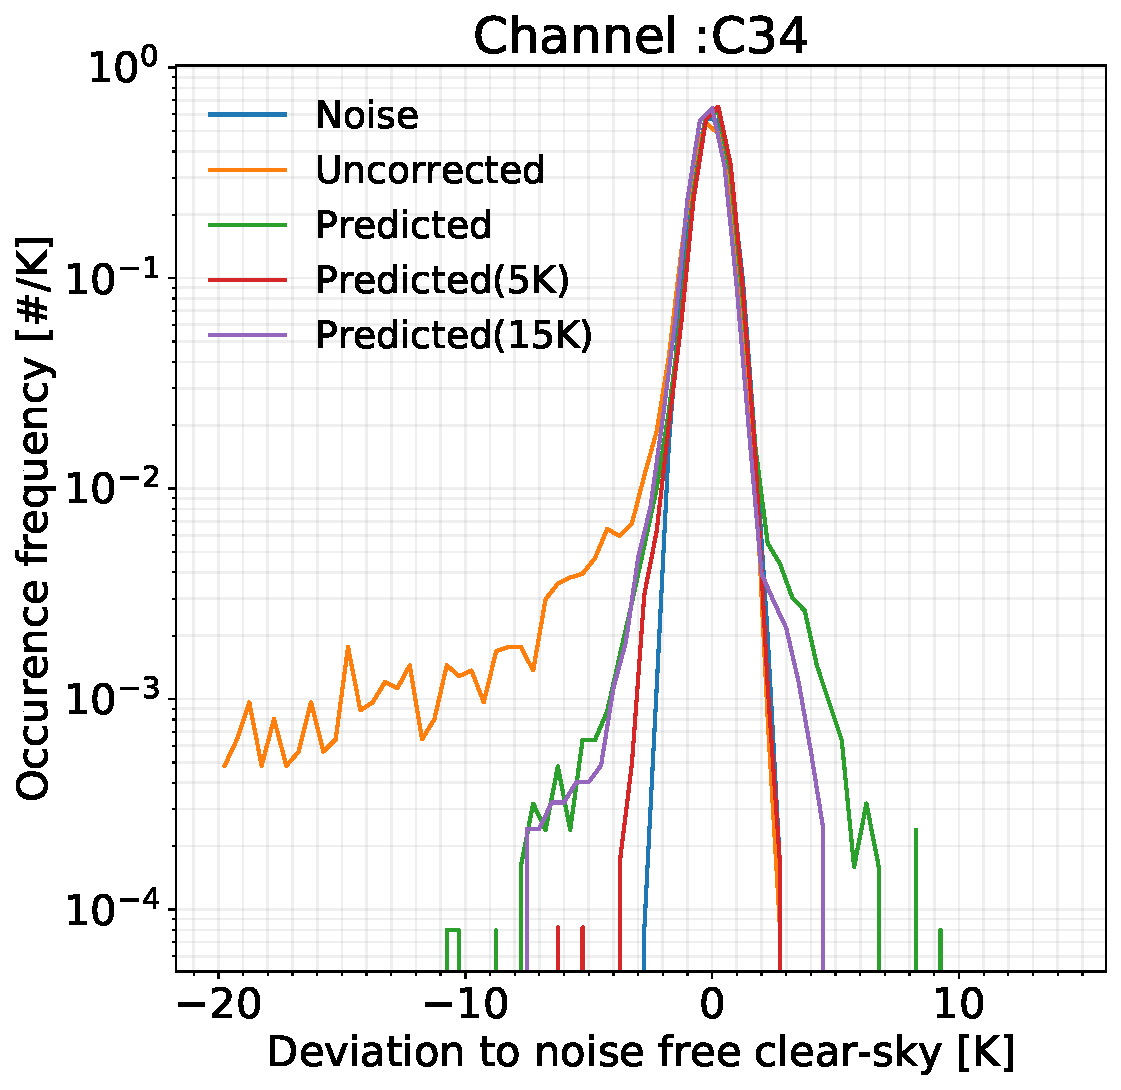
\includegraphics[width = 80mm]{Figures/AWS-34_single.pdf}	
	\caption{Error distributions for AWS-34 predictions. Label ``uncorrected'' represents the measurements, ``predicted'' denotes the entire dataset, while ``predicted(5\,K)'' and  ``predicted(15\,K)''  refers to the datasets where cases with cloud correction greater than 5\,K and 15\,K are excluded, respectively.}
	\label{fig:qrnn_C34_deviations}	
\end{figure}
In an analogy between the results from ICI channels, we perform a similar error distribution analysis. Fig.~\ref{fig:qrnn_C34_deviations} shows the error distributions of the measurements and predicted clear-sky TBs for AWS-34. The statistics corresponding to curves are provided in Table~\ref{tab:statistics_qrnn_aws}. The label ``Filtered'' represents the subset where all cases with correction greater than 5\,K(15\,K) are removed. The cloud impact in the uncorrected measurements is reflected in the high negative skewness (-10.30), however the  error distributions for the predictions are relatively symmetric. Removing cases with cloud correction greater than 5\,K, removes only 3.02\% of the data, but the errors reduce significantly. Infact, the standard deviation of predictions suggests that QRNN is successful in predicting the variability of noise-free simulations. 

Similar error statistics for other other 183\,GHz channels are also listed in Table~\ref{tab:statistics_qrnn_aws}. For channel AWS-32, the average bias and standard deviation in the prediction errors is is -1.34\,K and 5.91\,K respectively. However, after correction, the bias and standard deviation are -0.08\,K and 1.0\,K. A decrease in the skewness of error distributions is evident(from -7.48 to -1.52), but a relatively high values after prediction indicate presence of cases with partially-corrected cloud impact. For AWS-33, the predictions have slightly higher accuracy than AWS-32. The MAE in predictions is only 0.50\,K in comparison to 1.23\,K for the measurements. Similar results are also seen for AWS-35 and AWS-36. For both channels, the predictions are relatively more symmetric than the other channels. Also, it is worth to noting that when cases with 5\,K cloud correction are removed, the spread of predictions is narrower than noise. 

Overall the results demonstrate that QRNN is successful in predicting the clear-sky noise-free data for AWS-33, AWS-34, AWS-35 and AWS-36 and partially for AWS-32. The prediction error distributions are symmetric with low bias and standard deviation. The cases with high error are mostly associated with high cloud impact and constitute only a small fraction of the total dataset. Excluding such cases decreases the variability in the predictions and in fact the spread of errors for AWS-34, AWS-35 and AWS-36 is smaller than noise. Removal of cases with high cloud impact, increases the representation of cases in cloud-free conditions, and for such cases, QRNN predictions can be seen as a weighted mean between the two ``super-channels''. Since the noise in the two channels are stationary and uncorrelated, the predictions benefit from the additional information, but the noise component tends to cancel out. For AWS-32, QRNN is only partially successful in reducing the impact of hydrometeors. The prediction errors have significantly lower spread than the measurements, but cases with partially corrected cloud impact deteriorates the overall accuracy. Since 325\,GHz cannot provide a full coverage for hydrometeor impact in AWS-32, the testing data will inevitably contain cases for which QRNN has not trained for. Prediction for such \textit{out-of-distribution} cases would be inaccurate and highly uncertain. In such cases, the predictions should be used with caution. 

\begin{table}[t]
	\caption{Bias, mean absolute error(MAE), standard deviation(STD), and measure of skewness(Skewness) for error distributions of predictions AWS channels. Results are from QRNN-simple. The label ``All'' refers to the complete dataset, while in ``Filtered'', cases with cases with cloud correction greater than 5\,K(15\,K) are excluded from statistics. The fraction of cases removed by this filter are given in parentheses.}
	\label{tab:statistics_qrnn_aws}
	\begin{tabular}{llrr|rrr}
		\tophline
		&&\multicolumn{2}{c|}{Simulations}& \multicolumn{3}{c}{QRNN-simple} \\
		\cline{3-7}
		%		\hline
		&&   Clear-sky &   All-sky &   		 All &   Filtered(5K)& Filtered(15K) \\
		\middlehline
AWS-32    &Bias     &   -0.00 &         -1.34 &           -0.08 &       		-0.07(5.30\%) & -0.08(2.50\%) \\
          &MAE      &    0.36 &          1.58 &            0.62 &        		 0.53 		  &	0.57	\\
          &STD      &    0.45 &          5.91 &            1.00 &        		 0.74 		  & 0.85\\
          &Skewness &    0.02 &         -7.48 &           -1.52 &       		-1.63 		  & -2.01\\
		\middlehline
AWS-33	  &Bias     &   -0.00 &         -0.98 &            0.01 &                 0.00(4.08\%)& 0.00(1.75\%)\\
		  &MAE      &    0.36 &          1.23 &            0.50 &                 0.43 	      & 0.46\\
		  &STD      &    0.45 &          4.70 &            0.77 &                 0.57 	      & 0.64\\
		  &Skewness &    0.01 &         -8.76 &           -0.40 &                -0.90  	  & -1.00\\

		\middlehline
AWS-34	  &Bias    &    0.00 &         -0.68 &            0.02 &                0.01(3.02\%)& 0.01(1.11\%) \\
		  &MAE      &    0.50 &          1.08 &            0.53 &                 0.47 		 & 0.50\\
		  &STD      &    0.63 &          3.69 &            0.78 &                 0.62 		 & 0.70\\
		  &Skewness &    0.02 &        -10.30 &           -0.34 &                -0.49 		 &-0.76	\\
		 \middlehline
AWS-35	 & Bias     &    0.00 &         -0.42 &            0.01 &                 0.01(1.92\%) & 0.01(0.70\%) \\
		 &MAE       &    0.50 &          0.83 &            0.50 &                 0.47 		   & 0.49\\
		 &STD       &    0.63 &          2.65 &            0.71 &                 0.60         & 0.65\\
		 &Skewness  &    0.01 &        -12.45 &           -0.15 &                -0.15         &-0.26\\
		 \middlehline
AWS-36   &Bias     &    0.00 &         -0.27 &            0.02 &                 0.02(1.30\%) & 0.02(0.31\%)\\
		 &MAE      &    0.70 &          0.90 &            0.67 &                 0.64 		  & 0.06\\
		 &STD      &    0.88 &          2.06 &            0.91 &                 0.81 		  &0.85\\
		 &Skewness &   -0.01 &        -12.00 &           -0.51 &                -0.15 		  &-0.12\\	 
		\bottomhline				
	\end{tabular}
	\belowtable{} % Table Footnotes
\end{table}
\subsubsection{Uncertainty quantification}
%f
\begin{figure}[t]
	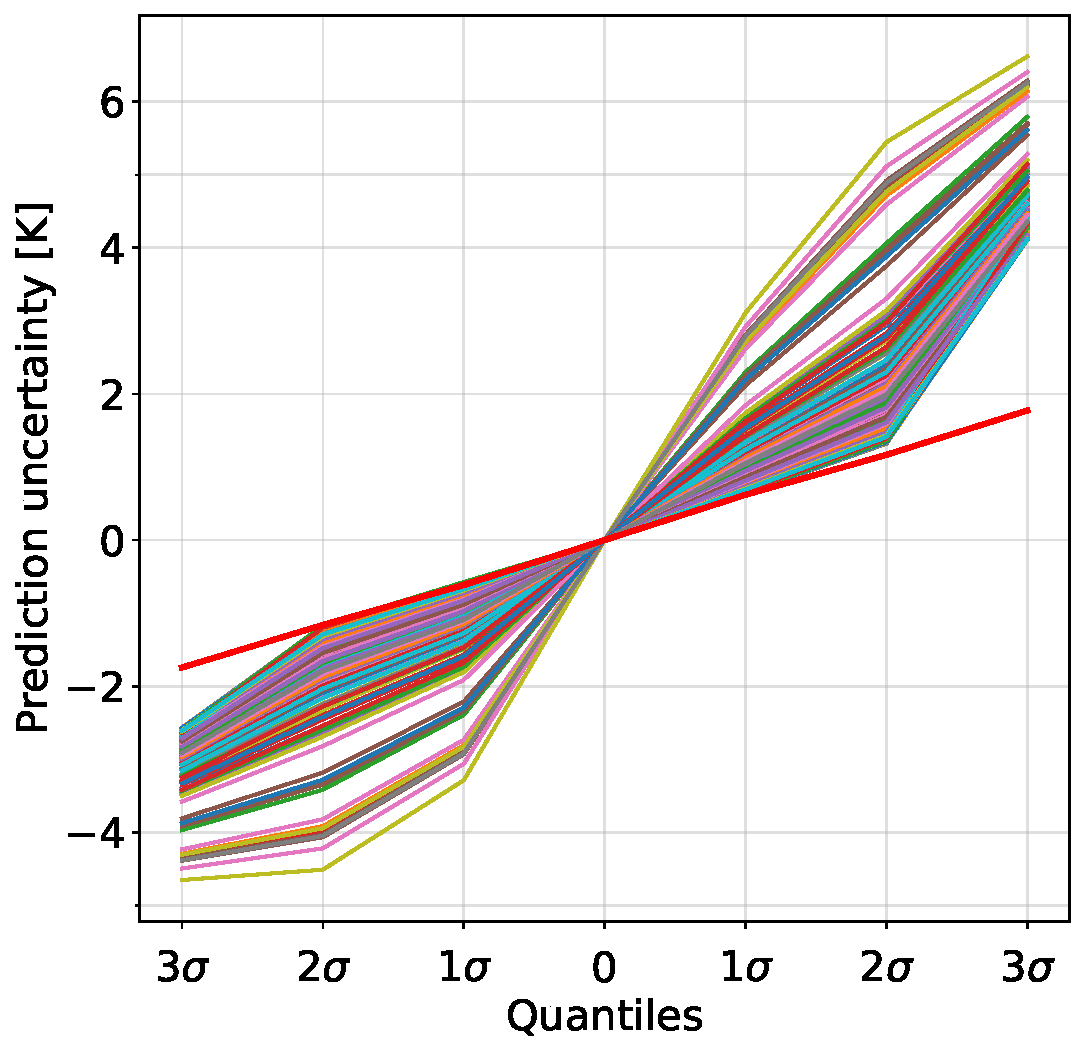
\includegraphics[width = 80mm]{Figures/prediction_uncertainty_aws-34.pdf}	
	\caption{The prediction uncertainty  for channel AWS-34  with respect to quantiles for randomly selected 1500 cases. The red line represents the uncertainty if underlying distribution is purely Gaussian with mean 270\,K and standard deviation 0.62\,K.}
	\label{fig:prediction_uncertainty_aws-34}	
\end{figure}
\begin{figure}[t]
	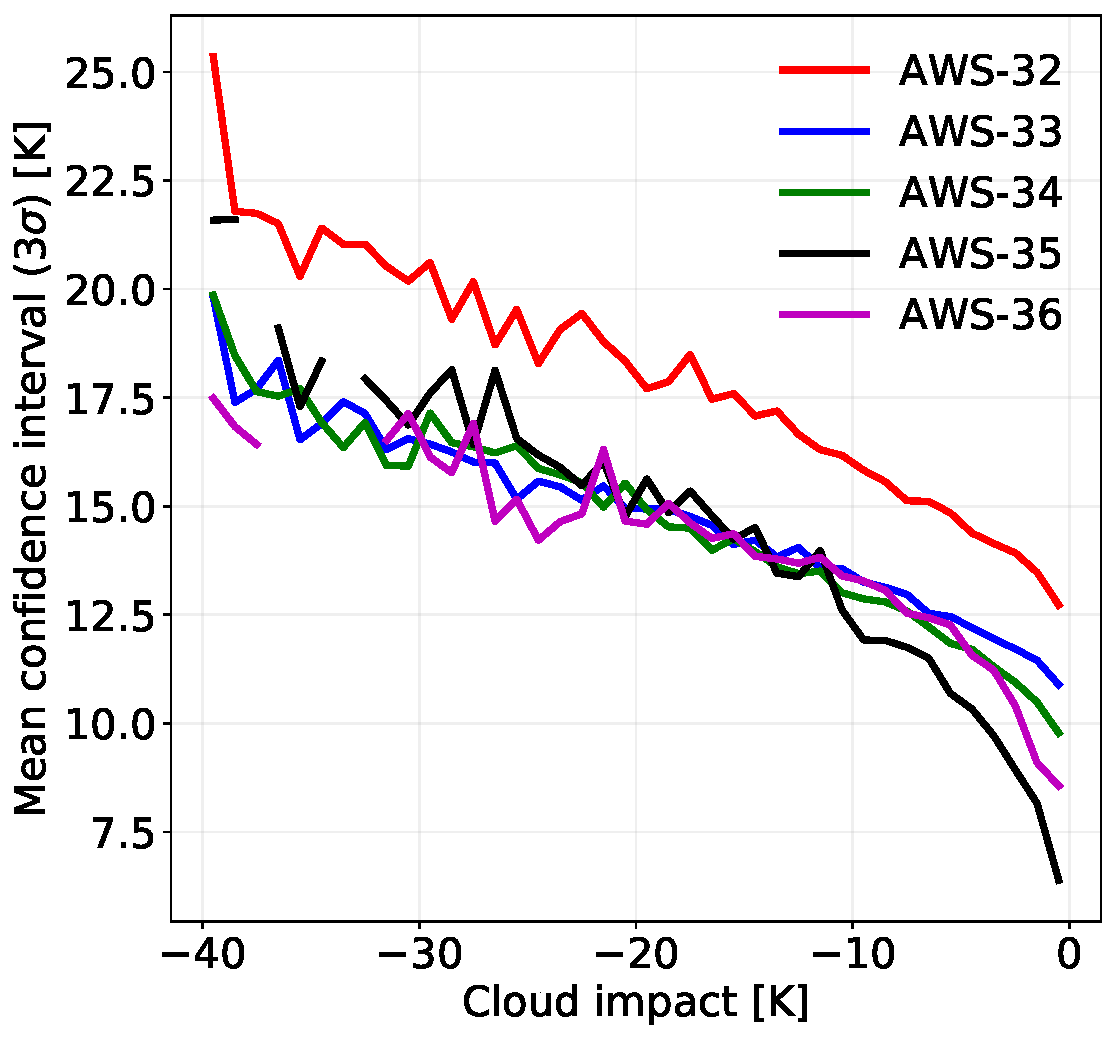
\includegraphics[width = 80mm]{Figures/cloud_impact_uncertainty_AWS.pdf}	
	\caption{The average confidence intervals (2$\sigma$) plotted against the magnitude of cloud impact for all AWS channels.}
	\label{fig:uncertainty_cloud_impact}	
\end{figure}

In this section, we analyse the uncertainty estimates obtained from QRNN.  Fig.~\ref{fig:prediction_uncertainty_aws-34} displays the prediction uncertainty in AWS-34 for different quantiles. The prediction uncertainty has been plotted as the deviation from the median value.  The different lines represent 1500 randomly chosen cases.  The red line represents the uncertainty in a hypothetical Gaussian distribution of $270\pm0.62$\,K, which is of the order of standard deviation of predictions for AWS-34 (see Table~\ref{tab:statistics_aws}). The high variability in the uncertainty estimates indicates that QRNN can successfully represent uncertainties for each case individually, rather than expressing them as a single measure for all cases. In the latter case, the uncertainty estimates would be concentrated along a narrow interval. Also, for majority of the cases, the prediction uncertainties are symmetric around the median, specially around  the 68\% ($\pm 1 \sigma$) and 94\% confidence interval ($\pm 2 \sigma$), suggesting that the posterior distribution follows a Gaussian distribution. 

In order to analyse the performance of QRNN with task difficulty, the interrelation between the uncertainty estimates and cloud impact was investigated. Here we assume that cloud impact is representative of task difficulty. Fig~\ref{fig:uncertainty_cloud_impact} displays the plot between mean uncertainty estimates for $2\sigma$ confidence interval and the cloud impact. For all five channels, the predictions with small or relatively low cloud signal have a low uncertainty or in other words have high sharpness. As fraction of cloud impact increases, the predictions become increasingly uncertain. However, this does not imply that the prediction accuracy is low. 

\section{Outlook and Conclusions}  %% \conclusions[modified heading if necessary]


%% The following commands are for the statements about the availability of data sets and/or software code corresponding to the manuscript.
%% It is strongly recommended to make use of these sections in case data sets and/or software code have been part of your research the article is based on.

\codeavailability{TEXT} %% use this section when having only software code available


\dataavailability{TEXT} %% use this section when having only data sets available


\codedataavailability{TEXT} %% use this section when having data sets and software code available


\sampleavailability{TEXT} %% use this section when having geoscientific samples available


\videosupplement{TEXT} %% use this section when having video supplements available


\appendix
\section{}    %% Appendix A

\subsection{}     %% Appendix A1, A2, etc.


\noappendix       %% use this to mark the end of the appendix section. Otherwise the figures might be numbered incorrectly (e.g. 10 instead of 1).

%% Regarding figures and tables in appendices, the following two options are possible depending on your general handling of figures and tables in the manuscript environment:

%% Option 1: If you sorted all figures and tables into the sections of the text, please also sort the appendix figures and appendix tables into the respective appendix sections.
%% They will be correctly named automatically.

%% Option 2: If you put all figures after the reference list, please insert appendix tables and figures after the normal tables and figures.
%% To rename them correctly to A1, A2, etc., please add the following commands in front of them:

\appendixfigures  %% needs to be added in front of appendix figures

\appendixtables   %% needs to be added in front of appendix tables

%% Please add \clearpage between each table and/or figure. Further guidelines on figures and tables can be found below.



\authorcontribution{TEXT} %% this section is mandatory

\competinginterests{TEXT} %% this section is mandatory even if you declare that no competing interests are present

\disclaimer{TEXT} %% optional section

\begin{acknowledgements}
TEXT
\end{acknowledgements}




%% REFERENCES


 \bibliographystyle{copernicus}
 \bibliography{references.bib}

\end{document}
